%不需修改部分
\documentclass[UTF8]{ctexart}  %使用中文版的article文档类型排版,并选择UTF8编码格式
\usepackage{algorithm}
\usepackage{algorithmic}
\usepackage{amsmath}
\usepackage[colorlinks,linkcolor=black,anchorcolor=blue,citecolor=green]{hyperref}    %修改特定内容的颜色
\usepackage{enumerate}                      %条目包
\usepackage{float}                          %固定表格位置
\usepackage{graphicx}                       %图片包
\usepackage{float}                          %设置图片浮动位置的宏包
\usepackage{subfigure}                      %插入多图时用子图显示的宏包
\usepackage{titlesec}                       %自定义多级标题格式的宏包
\usepackage{geometry}
\usepackage{wrapfig}
\pagestyle{plain}						    %显示页码
\RequirePackage{fix-cm}                     
\usepackage{longtable}
\usepackage{listings}
\usepackage{setspace}
\usepackage{xcolor}
\usepackage{caption}
\usepackage{diagbox}
\usepackage{multirow} %合并多行单元格的宏包
\usepackage{longtable} %不宽但很长的表格可以用longtable宏包来进行分页显示
\usepackage{array} %一般用于数学公式中对数组或矩阵的排版
\usepackage{makecell}% makecell命令对表格单元格中的数据进行一些变换的控制。我们可以使用 \ 命令进行换行,也可以使用p{(宽度)}选项控制列表的宽度
\usepackage{threeparttable} %制作三线表格
\usepackage{booktabs}%s三线表格中的上中下直线线型设置宏包,在这个包中水平线被教程\toprule、midrule、buttomrule。

%标题格式,可根据需要进行修改
\titleformat{\section}[block]{\Large\bfseries}{\arabic{section}.}{1em}{}[]
\titleformat{\subsection}[block]{\large\itshape\bfseries}{\arabic{section}.\arabic{subsection}}{1em}{}[]
\titleformat{\subsubsection}[block]{\normalsize\bfseries}{\arabic{section}.\arabic{subsection}.\arabic{subsubsection}}{1em}{}[]
\titleformat{\paragraph}[block]{\small\bfseries}{[\arabic{paragraph}]}{1em}{}[]

\geometry{a4paper,left=2cm,right=2cm,top=2cm,bottom=2cm}



\begin{document}

\begin{titlepage} %制作封面
        \heiti
        \vspace*{100pt}
        \begin{center}
            \fontsize{48pt}{0} 人\quad 工\quad 智\quad 能\quad 导\quad 论\\
            \vspace*{36pt}
            \fontsize{36pt}{0}{第\quad 二\quad 次\quad 大\quad 作\quad 业\quad 实\quad 验\quad 报\quad 告}\\
            \vspace*{48pt}
            \LARGE(2023\ -\ 2024\ 学年度\quad 春季学期)\\
            \vspace*{48pt}

            \LARGE 实验名称\ \ \underline{\makebox[300pt]{智能车运送货物}}\\
            \vspace*{72pt}

            \heiti\Large 姓名\ \ \underline{\makebox[168pt]{\songti 张章}}\\
            \heiti\Large 学号\ \ \underline{\makebox[168pt]{\songti 2023010916}}\\
            \heiti\Large 院系\ \ \underline{\makebox[168pt]{\songti 自动化系}}\\
            \heiti\Large 教师\ \ \underline{\makebox[168pt]{\songti 张长水}}\\
			\heiti\Large 时间\ \ \underline{\makebox[168pt]{\songti 2024/5/30}}\\
        \end{center}
\end{titlepage}

\tableofcontents %插入目录
\thispagestyle{empty}

\newpage %正文
\section{摘要}
本实验旨在设计一种算法完成对多智能体的路径规划,使得各个智能体能够无冲突地完成将货物从一个仓库转移至另一个仓库的
任务。在本实验中,作者设计了一种方法将该问题转换成一系列经典的多智能体路径规划问题,并使用基于冲突的搜索算法解决
这一系列的多智能体规划问题。实验结果和项目仓库已经上传至Githuhb,请通过以下链接查看:https://github.com/SuoRuGithub/agents-deliver-goods/tree/main

\section{定义实验任务}
大作业题目并没有对本次实验要完成的内容做出详细的指示,因此在介绍实验方法前,作者将先对实验任务进行定义。

本次实验中,我们将随机生成一幅地图,地图上分布着由等大的小正方形组成的障碍物以及仓库$A$和仓库$B$。我们假设在初始
状态下在仓库$A$存在着$N$件货物,地图形状如图1所示。$M$辆无人货车随机地分布在地图上的各处,它们在单位时间内能够向上下左右四个方向移动
的距离固定,每辆货车最多只能装载一个货物。考虑到实际情况,我们认为$M$应当小于$N$。因此,我们的任务可以定义为:规划
所有小车的路线,使它们在两个仓库之间来回折返,运送货物,直到所有的货物都从仓库$A$移动至$B$仓库为止。且这些小车的路线应当满足:
1)路线要能自主避开障碍物;2)这些路线两两之间并无冲突,即两辆货车不会在同一时间占据同一个位置,也不会在某一时刻
彼此交换位置,如图2所示;3)在满足前两个条件的前提下,路径花费的代价应该尽可能少,也就是所有小车移动距离的总和最小。


\begin{figure}[H]
    \centering
    \centering
    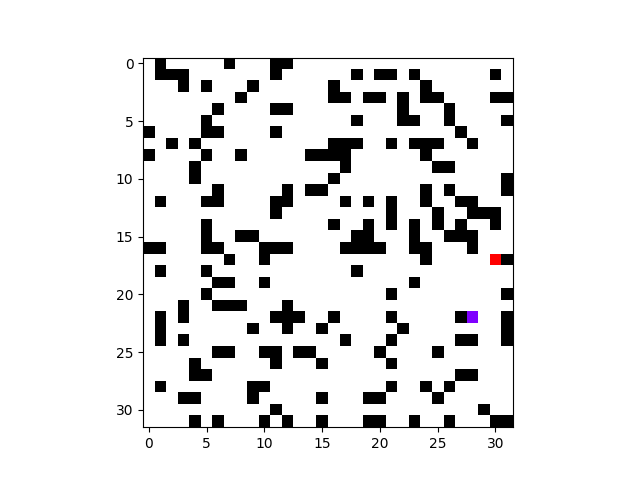
\includegraphics[width=0.6\textwidth, keepaspectratio]{fig1.png}
    \captionsetup{font=footnotesize}
    \caption{一个地图的示例,图中黑色部分表示障碍物,紫色方格表示仓库$A$,红色方格表示仓库$B$}
    \label{figure1}
\end{figure}

\begin{figure}[H]
    \centering
    \centering
    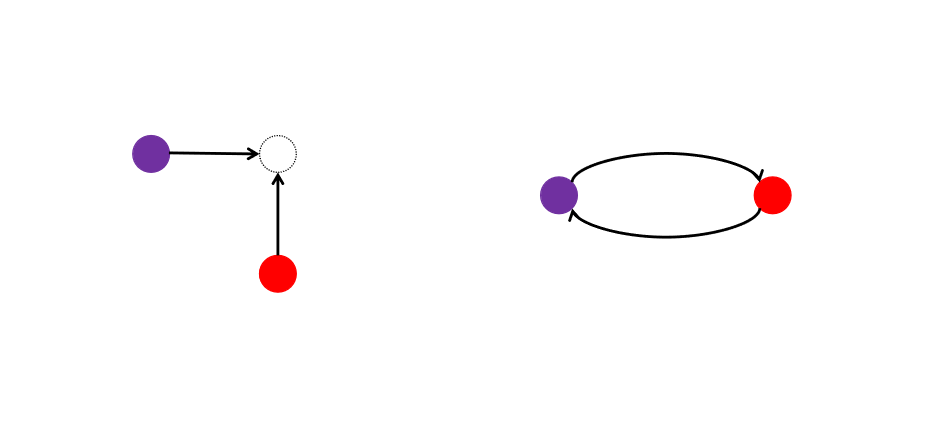
\includegraphics[width=0.6\textwidth, keepaspectratio]{fig2.png}
    \captionsetup{font=footnotesize}
    \caption{图中展示了两种冲突的可能,左侧表示两小车在同一时刻占据同一位置,右侧表示两小车在某一时刻互换位置}
    \label{figure1}
\end{figure}

% \section{实验目标}
\section{实验方法}
本次实验中,作者将实验的任务分解成一系列经典的多智能体路径规划(Multiple Agent Path Finding, 以下简称MAPF)问题,
然后通过使用基于冲突的搜索(Conflicts-Based Search, 以下简称CBS)算法解决这些MAPF问题,得到整个问题的解。CBS是一种
两层算法,底层寻找单个智能体的最佳路径,顶层负责处理路径之间的冲突。作者在CBS的底层使用了时空联合的A*(Space-Time A*)
算法进行单个智能体的寻路。
\subsection{全局算法}
经典的MAPF问题需要规划所有智能体的路径,使得它们能够无冲突地从起始到达目标位置。与之相比,本次实验中小车需要在两个
仓库之间来回折返,终点位置也在不断变化,因此作者要先将本实验问题转化成一系列经典的MAPF问题。

小车是否载货和仓库$A$是否还有剩余货物的情况有以下几种组合:1)小车没货,仓库A有货 2)小车有货,仓库A有货 3)小车有货,仓库A没货 4)小车没货,仓库A没货。
组合的情况决定了单个小车的状态:1)小车需要从当前位置去仓库$A$取货 2)与3)小车需要从当前位置去仓库$B$送货 4)任务已经完成,无需移动。

现在我们将所有小车记作$\bf c$,在某一时刻$t_n$,所有的小车的状态记作$\bf x_n$,所有小车完成当前任务之后的状态记作$\bf x_{n+1}$(此时我们假设先到达目标
位置的小车在到达之后暂停运动,而不会更新自己的状态),可以发现,从$\bf x_n$到$\bf x_{n+1}$的过程是一个标准的MAPF问题,我们可以基于CBS算法,计算得到它的
解$\bf S$。现在假设在上述解$\bf S$中,小车$c_i$在$t_{n+1}$时刻率先到达了自己的目标位置,并更新自己的状态为$\displaystyle x_n^{(i)\prime}$,此时,上述解并没有被
全部遍历完,我们将已经遍历的部分解记作$\bf S^{\prime}$,该小车更新后整体的状态变成$\bf x_n^{\prime}$,整体目标状态变成$\bf x_{n+1}^{\prime}$,可以看到这又是
一个经典的MAPF问题。如此重复,当仓库$A$已经没有货物且所有小车都不再装载货物时,算法结束。将所有的部分解拼接在一起,我们就一个得到全局解$\bf G$。按照上述的思路,我们算法的过程可以这样描述:

% 算法伪代码块
\begin{algorithm}[H]
    \renewcommand{\algorithmicrequire}{\textbf{Input:}}
	\renewcommand{\algorithmicensure}{\textbf{Output:}}
    \caption{Get Global Solution}
    \label{alg:example}
    \begin{algorithmic}[1]
        \REQUIRE 

            game map matrix: $\bf M$,

            a list of all agents' states: $\bf A$
        \ENSURE
            Global Solution $\bf G$, a two-dimension array of coordinates.

        \STATE initialize Global Solution $\bf G$  
        \WHILE{not every agent has concluded its task}
            \STATE caculate Partial Solution $\bf P$ with CBS algorithm
            \STATE concatenate $\bf P $ to $\bf G$
            \STATE update states of all agents.
        \ENDWHILE
        \RETURN $\bf G$
    \end{algorithmic}
\end{algorithm}


\subsection{局部解算法——CBS算法}
在上面,我们已经将本次任务转化成一系列经典的MAPF问题,我们使用CBS算法来解决MAPF问题。

CBS算法是一种两层算法,底层使用传统的寻路算法为单个智能体规划路径,顶层则通过维护一个冲突树来解决各个智能体路径之间的冲突。
为了更详细的介绍CBS算法,我们先规定以下术语:$path$表示单个智能体找到的路径,$solution$为所有智能体路径的集合,$cost$表示当前$solution$的总成本,
$conflict$表示路径之间存在的冲突,$constraint$表示由冲突产生的对单个智能体寻路的约束,由一个三元组$( i, \bf v, t)$表示,即智能体$i$在
$t$时刻不允许占据顶点$\bf v$的位置。

我们先来介绍算法的顶层,顶层算法维护一个$open$表,其中每一个结点都包含一组$constraint$,一个$solution$及其总成本$cost$。算法刚开始时,我们不给
智能体添加约束,生成一个$solution$并将结点放入$open$表中。此后,我们每一次都从$open$表中取出成本最低的结点,如果该结点的解没有冲突,则说明$solution$已经被找到了
,如果有冲突,我们将通过该冲突生成两个约束,由此原来的结点就会分叉成两个子结点(见图2),每个子节点在继承父节点已有的$constraint$的基础上加入了新的约束。我们将子
节点重新放入$open$表中,重复上述过程,直到没有约束为止。

\begin{figure}[H]
    \centering
    \centering
    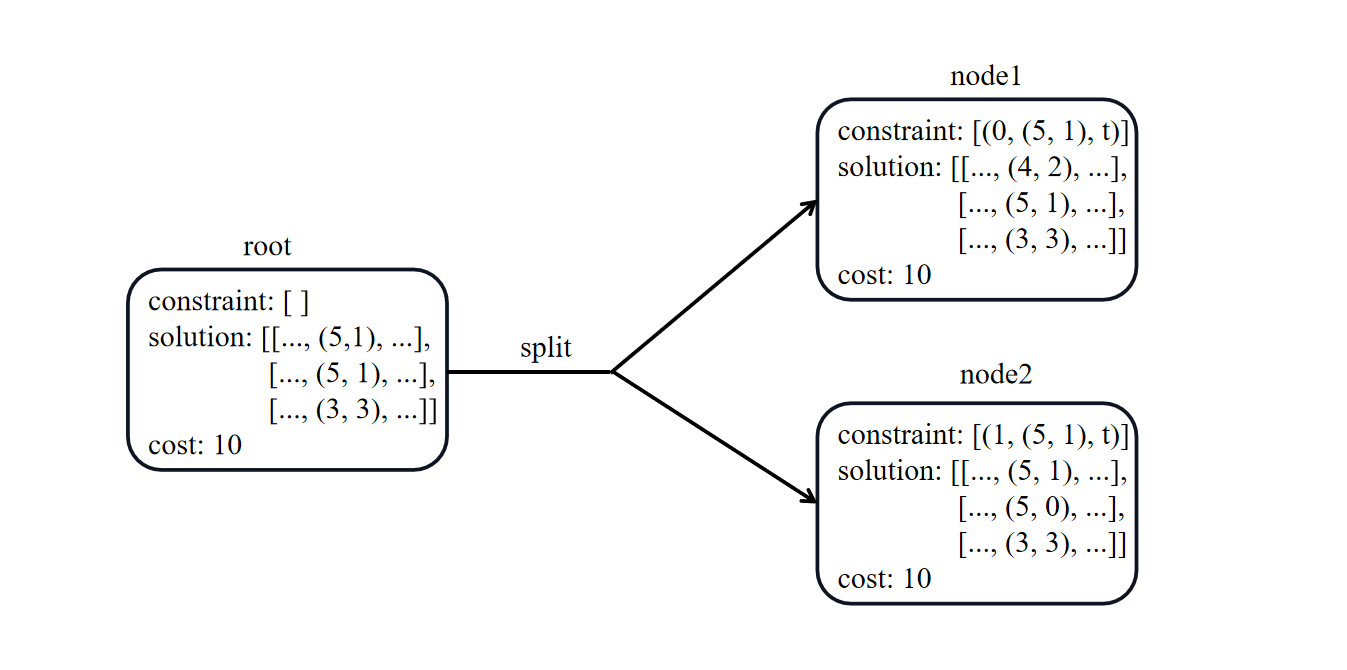
\includegraphics[width=0.6\textwidth, keepaspectratio]{fig3.png}
    \captionsetup{font=footnotesize}
    \caption{根节点中智能体0和智能体1存在路径上的冲突,由此产生了两个约束,通过这两个约束重新生成结点1和结点2}
    \label{figure1}
\end{figure}

\begin{algorithm}[H]
    \renewcommand{\algorithmicrequire}{\textbf{Input:}}
	\renewcommand{\algorithmicensure}{\textbf{Output:}}
    \caption{Get Partial Solution}
    \label{alg:example}
    \begin{algorithmic}[2]
        \REQUIRE 
            game map matrix: $\bf M$,

            a list of all agents' states: $\bf A$
        \ENSURE
            Partial Solution $\bf P$, a two-dimension array of coordinates.

        // definition of Node: 

        // - class attributes: constraints, cost, solution(may include collisions)
        
        // - class methods: get first collision, split collision to constraints, 

        \STATE initialize Partial Solution $\bf G$  
        \STATE initialize $open list$
        \STATE initialize $root node$, push it in $open list$
        \WHILE{$open list$ is not empty}
            \STATE get least costly node $n$ from $open list$
            \STATE remove $n$ from $open list$
            \IF {node $n$ has no collision:}
                \STATE the partial solution has already been founded
            \ELSE
                \STATE get constraints $\bf c$ based on the first collision
                \FOR {constraint $c$ in constraints $\bf c$}
                    \STATE new constriants $\gets$ old constraints of node + $c$
                    \STATE create new node based on new constriants
                    \STATE push new node in $open list$
                \ENDFOR
            \ENDIF
        \ENDWHILE
    \end{algorithmic}
\end{algorithm}


\subsection{CBS的底层寻路——时空联合的A*算法}
接下来我们介绍本次实验中CBS算法的底层部分,也就是为单个智能体寻找路径的算法。诸如A*算法和Dijkstra算法
都能很好地完成寻路的任务,但是它们的缺陷在于它们处理的地图不能随着时间发生变化。在本次实验中,每个小车
的移动需要考虑其他小车的位置,也就是地图上的障碍物会发生变化。因此,本次实验中CBS的底层寻路算法需要使用
时空联合的A*算法而并非传统A*算法。


\begin{algorithm}[H]
    \renewcommand{\algorithmicrequire}{\textbf{Input:}}
	\renewcommand{\algorithmicensure}{\textbf{Output:}}
    \caption{Space-Time A* Path Finding}
    \label{alg:example}
    \begin{algorithmic}[3]
        \REQUIRE 
            Game map matrix: $\bf M$,

            A single agent: $a$

            A constraints table $\bf c$ 
            
        \ENSURE
            A optimal path of agent $a$

        // definition of Node: (diffrent from Node in CBS algorithm)

        // - class attributes: current position, target, parent node, time, total cost      

        // - class methods: find neighbours, return all avilable position for next time
        

        \STATE initialize $open list$  
        \STATE initialize $closed list$
        \STATE initialize $root node$, push it in $open list$
        \WHILE{$open list$ is not empty}
            \STATE get least costly node $n$ from $open list$
            \STATE remove $n$ from $open list$
            \STATE get $neighbours$  of node
            \FOR{$neighbour$ in $neighbours$}
                \IF{position of $neighbour$ equals target of node}
                    \STATE path $\bf p$ has already been founded
                \ELSE
                    \STATE add $neighbour$ in $open list$
                \ENDIF
            \ENDFOR
        \ENDWHILE
    \end{algorithmic}
\end{algorithm}

\section{实验结果展示}
由于作者不会使用\LaTeX 插入动图,实验结果展示请看上传的作业文件中的/Demo文件夹,或在项目的Github仓库:https://github.com/SuoRuGithub/agents-deliver-goods/tree/main
中查看。
\section{回顾与展望}
本实验利用CBS算法,解决了货车运货的实际问题。不过,本次实验仍然存在着许多不足。首先,实验代码的鲁棒性仍然有待提高,实验中仍然会偶尔出现找不到解的情况。其次,实验采用的算法较为耗时,这使得目前的实验仍然局限于小尺寸的地图上。

在前期调查的过程中,作者了解到MAPF问题解决方法主要有集中式规划的方法与分布式执行的方法。本实验中采用的CBS算法就是集中式
规划方法中的一种情况,它仍然是以搜索算法作为基础的。在未来,作者希望能够使用基于强化学习的分布式执行的算法继续完善本次实验。
%\pagenumbering{arabic}%页码

%分点列举
% \begin{itemize}

%\item{}

%\end{itemize}

\end{document}  %结束写文章